\documentclass[etudiants]{support-iutrs}
\usepackage{pdfpages}

\infos{Steve Benedik, Kévin Hagner, Jean Meyblum}{E31}{TD 1}

\sujet{}
\titre{Planification des tâches}

\begin{document}

\header

\section{Estimation des charges} 
Nous avons hésité entre les méthodes \emph{par analogie} et \emph{analytique} pour réaliser l'estimation des charges.
Cependant, le \emph{diagramme de Gantt} traite déjà partiellement la méthode \emph{analytique}. 
C'est pour cette raison que nous nous sommes tourné vers la méthode \emph{analogique}, afin d'avoir deux résultats et de pouvoir les comparer entre eux. 

\subsection{Estimation par analogie}

Pour la réalisation des estimations de temps nécessaire à la réussite de ce projet,
nous avons donc choisi la methode d''\emph{estimation par analogie}.
Elle correspond à calculer le temps nécéssaire à l'aide d'une proportion des différentes étapes du projet. 

\begin{tabular}{|l l|l|l|}
\hline
&& Durée proportionnelle & Durée concrète \\
\hline
Opportunité & Étude préalable & 10\% & 60h \\
\hline
Élaboration & Conception de la solution détaillée & 30\% & 180h \\
\hline
Construction & Développement & 50\% & 300h \\
\hline
Transition & Mise en œuvre & 10\% & 60h \\
\hline
\end{tabular}

Avec cette méthode, nous avons une estimation de travail de $60 + 180 + 300 + 60 = 600$ heures. 


\subsection{Difficultés encourues} 
Le principal problème se situait au niveau de la prise en main de \emph{MS Project}…

Si non, l'estimation du temps de réalisation des fonctionnalités a aussi été un problème. 
En effet, le manque d'expérience dans le domaine du travail en équipe nous empêche de bien définir si nos enchainements entre la réalisation des fonctionnalités se  déroulerons bien comme prévu, et si nous arriverons à travailler ensemble efficacement. 

Le deuxième problème dans l'estimation vient de notre manque d'expérience en tant que programmeur :
L'instabilité des connaissances acquises nous fera peut être perdre du temps dans l'apprentissage de quelque chose qu'on aura estimé plus simple à assimiler. 

Enfin, le découpage du projet en tâches n'a pas été trop problématique. 
Si ce n'est qu'au début leurs nombres c'était révélés un peu trop important,
et que nous avions du en fusionner quelques unes. 

\section{Planification de T3}

\emph{Le contenu de cette partie est présenté en annexe.
	Il s'agit d'une exportation de notre réalisation sur \emph{MS Project}.}

\newpage{}
\section{Cycle de vie du T3}
Nous avons choisi d'adapter notre projet au cycle de vie \textbf{ICAR} pour deux principales raisons : 

La première, c'est que la structure même du T3 nous impose presque son utilisation :
en effet, nous devons livrer un cahier des charges, puis une analyse fonctionnelle, suivie d'un prototype, et enfin de la version finale. 
Un cycle en V, par exemple aurait été assez difficile à tenir avec ce mode de fonctionnement vu que toutes les étapes « se mélangent » un peu. 

La seconde vient justement de la structure claire qu'elle exige. 
En effet, tout le projet est hiérarchiser (on doit, par exemple d'abord finir le cahier des charge avant de s'attaquer à l'analyse fonctionnelle). 
De cette façon, l'effet didactique du projet est amplifié car nous apprenons d'abord à rédiger correctement, puis à coder. 
De plus le contrôle est plus efficace ce qui permet de nous corriger assez rapidement en cas d'erreur.

\section{Conclusion}
\emph{MS Project} nous a calculé le temps de développement à \textbf{253h}. 
Avec notre estimation par analogie, nous avons trouvé un temps consacré au développement de \textbf{300h}. 
Nous pouvons donc dire que globalement, les résultat concordent. 
Ceux-ci peuvent donc être fiable, et le temps réel devrait se situé entre 253 et 300h de codage. 

\newpage{}
\section{Annexe — Résultat \emph{MS Project}}

\begin{figure}[h!]
 \centering
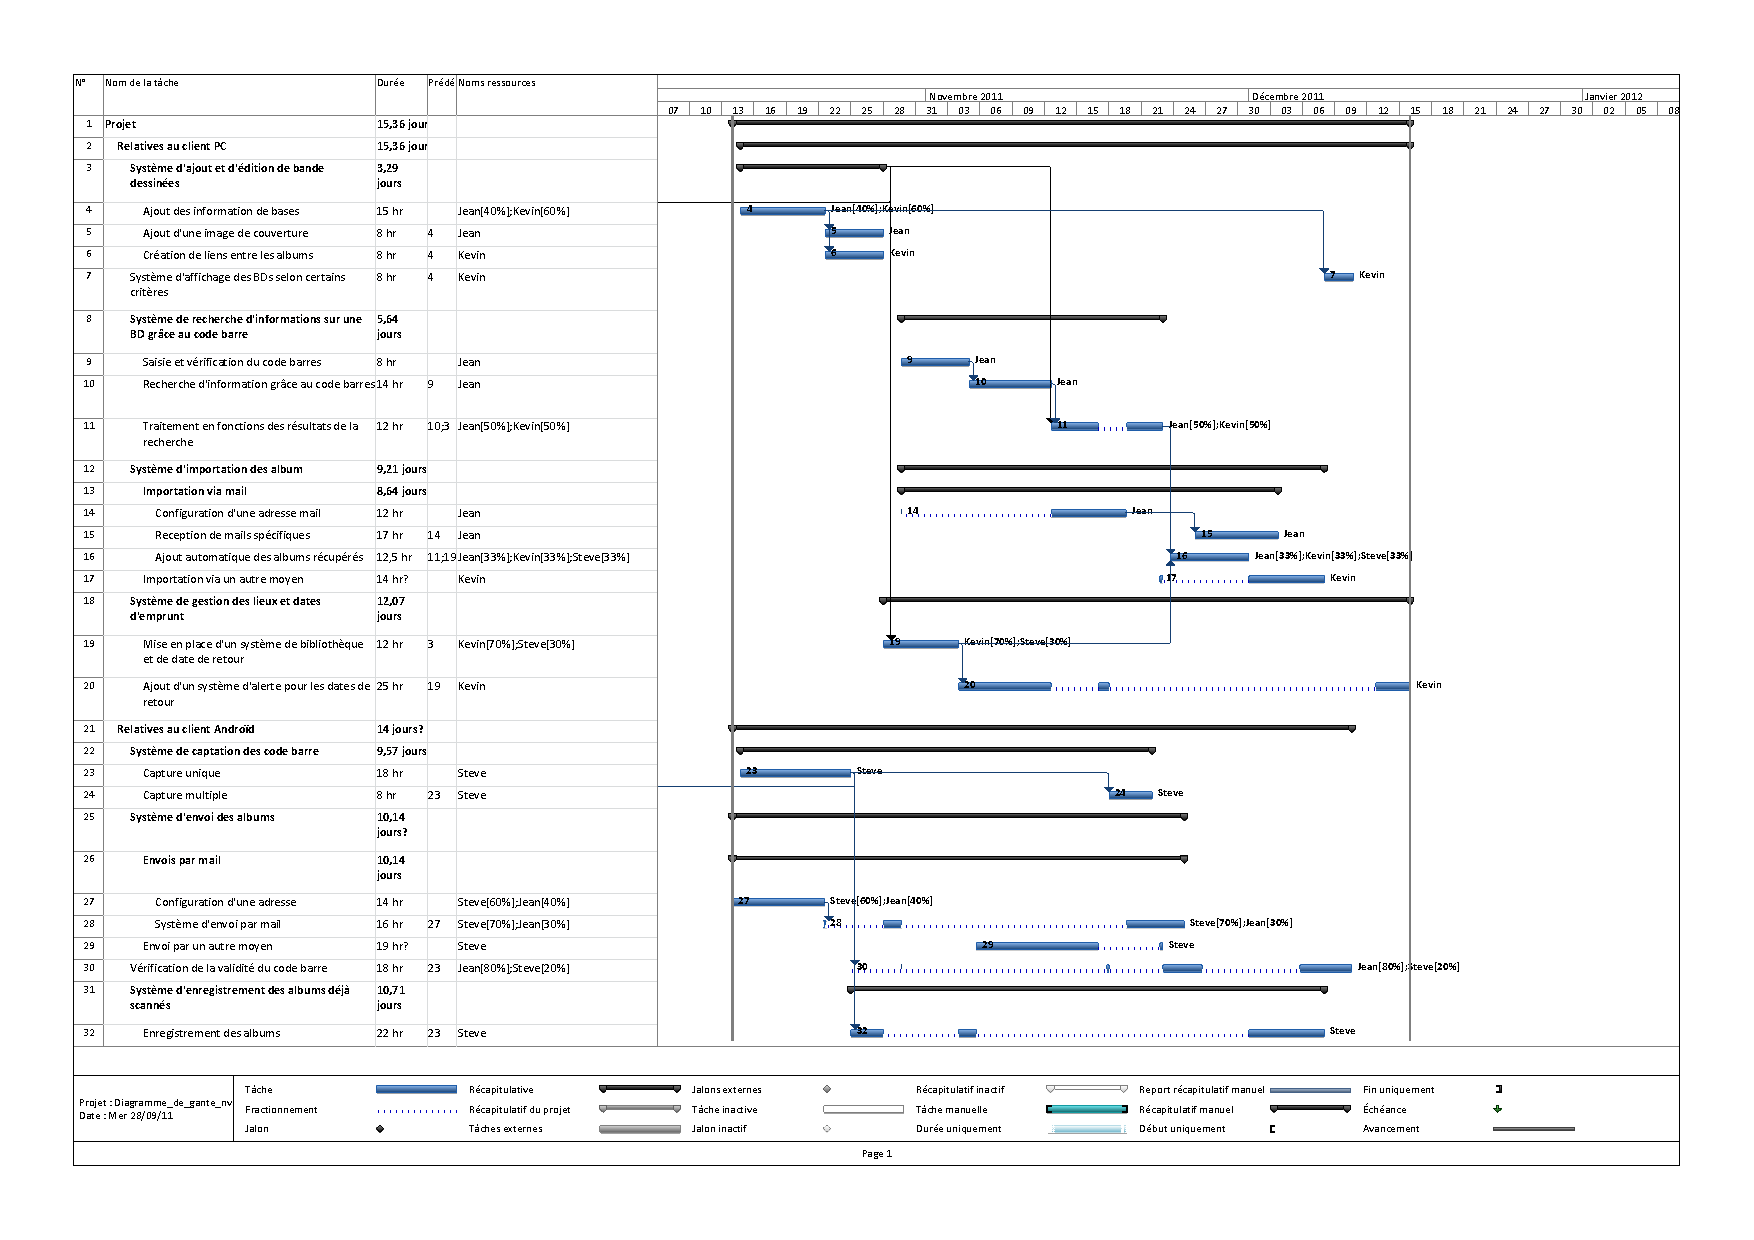
\includegraphics[angle=90, width=16cm]{diagramme_gante.pdf}
\end{figure} 

%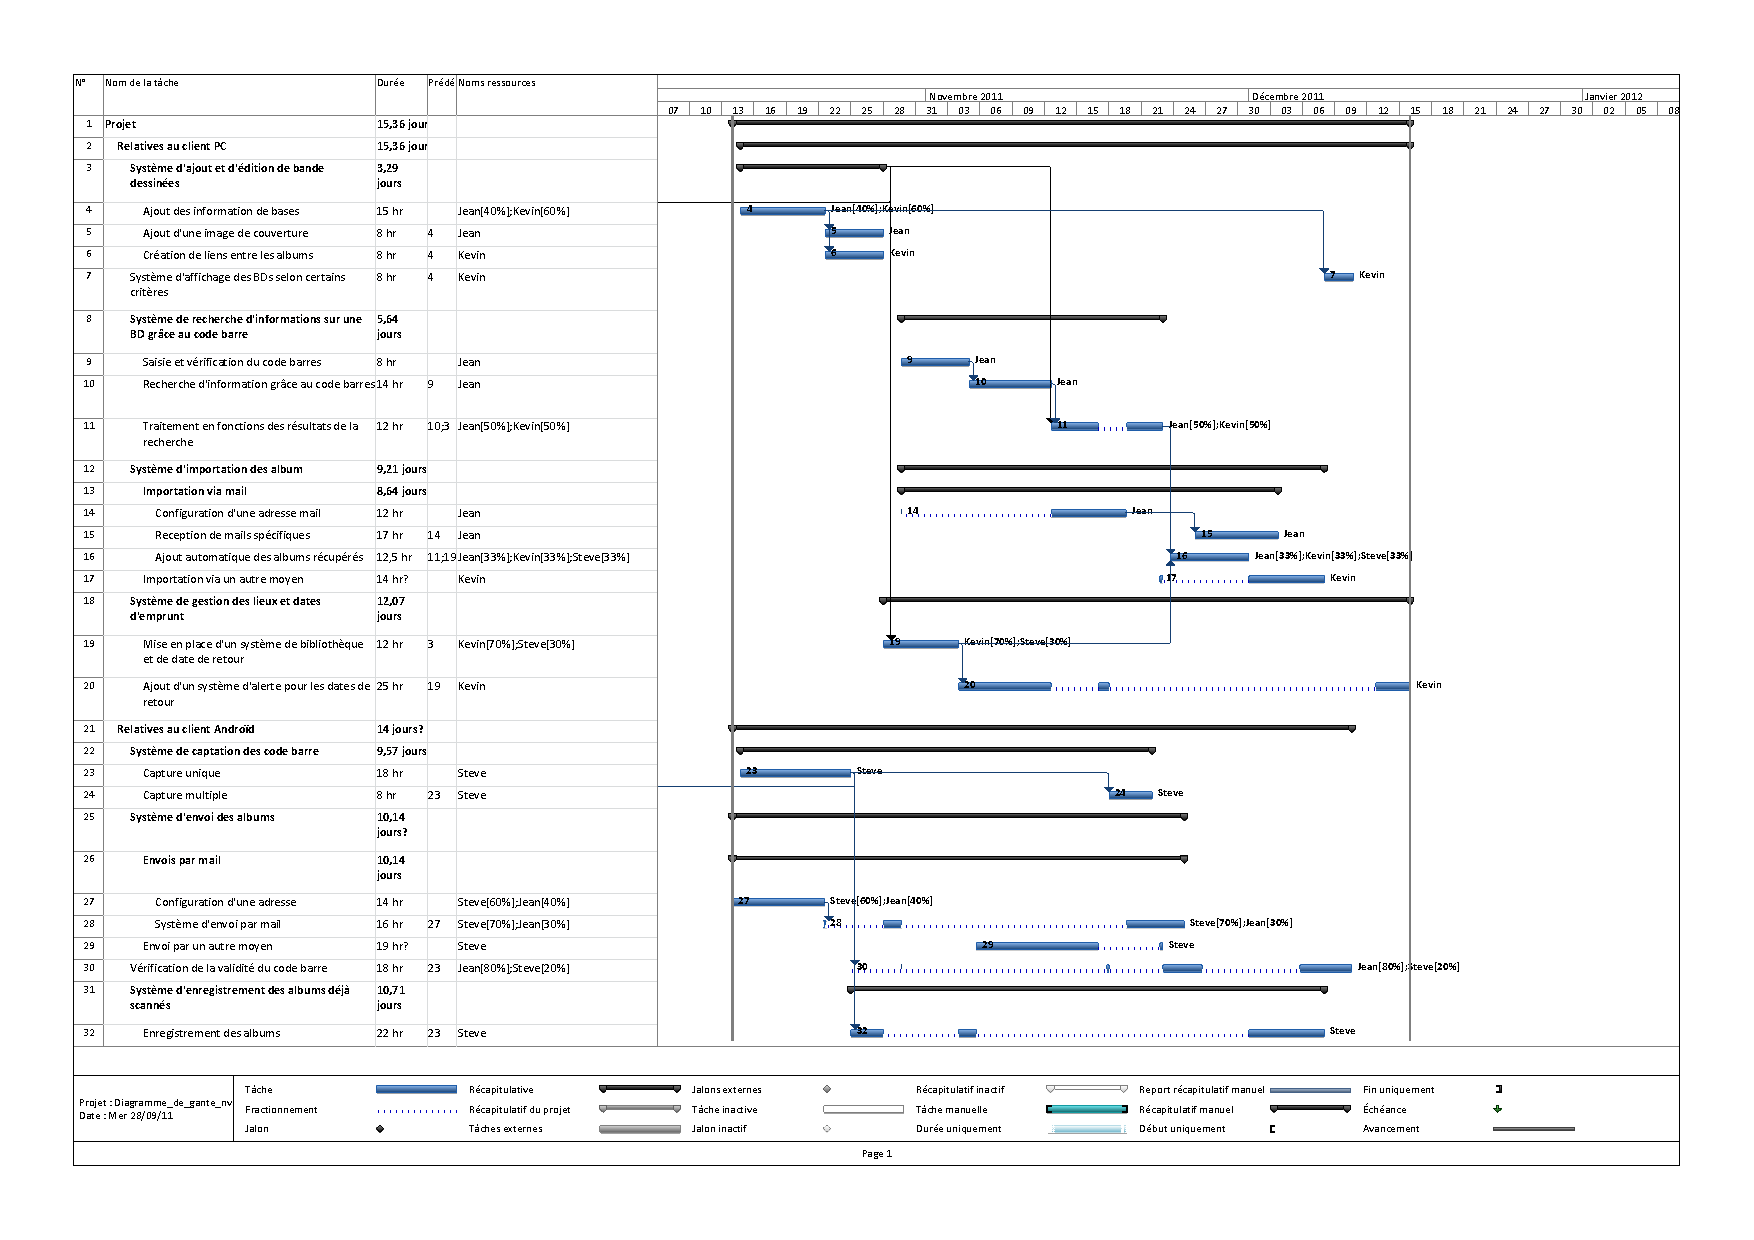
\includepdf[landscape=true, addtotoc={1,section,1,Coucou,Résultat \emph{MS Project}]{diagramme_gante.pdf}
%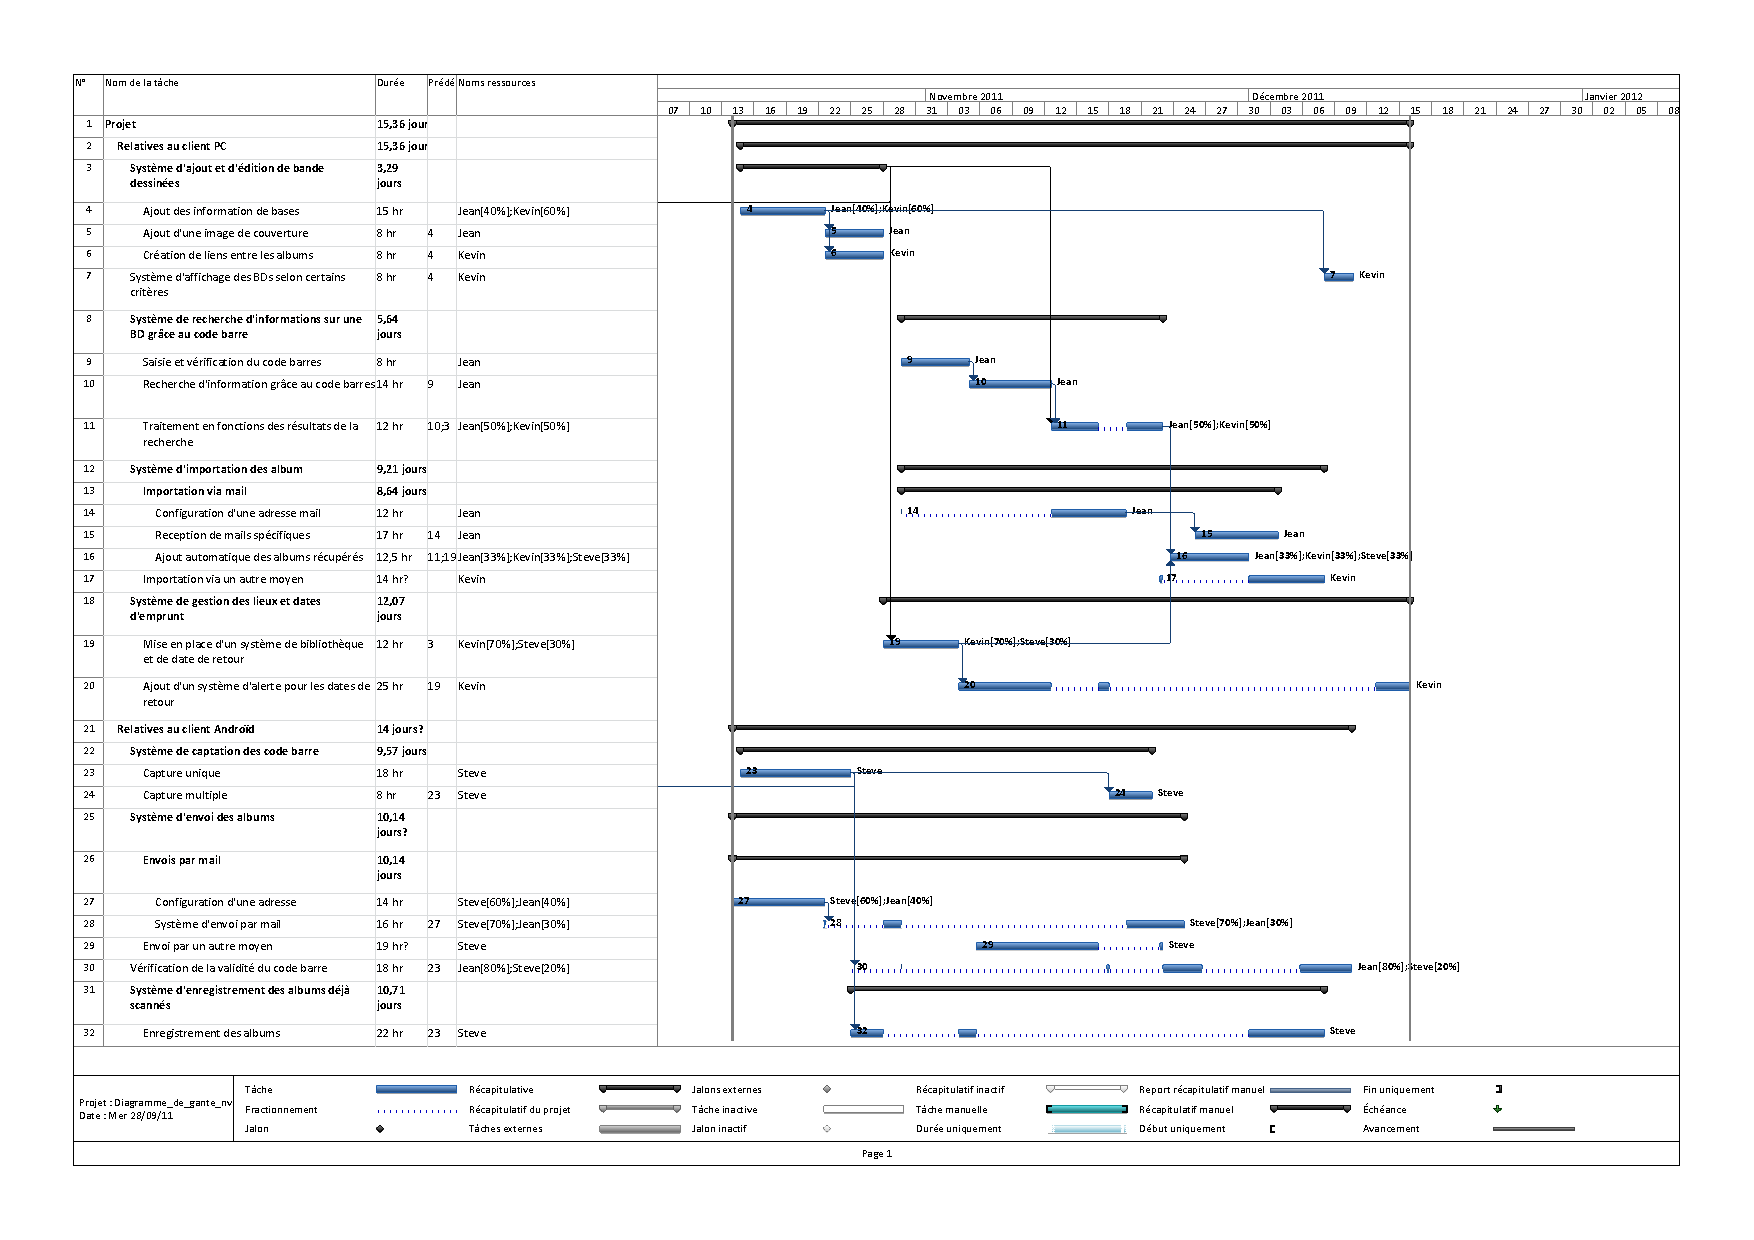
\includepdf[pagecommand={}, landscape=true, scale=1, addtotoc={1,section,1,Truc cool,Résultat \emph{MS Project}}]{diagramme_gante.pdf}


\end{document}
